\chapter{Introduction}
Lors du développement de notre application Getting Things Done, nous avons utilisé plusieurs technologies permettant la manipulation d'objets distribués et de services distants dont certaines ont été abordées en cours .\\
Ce livrable fera donc office de synthèse concernant le partage d'objets et l'utisation de services distants au sein de notre projet.\\
Nous commencerons par détailler l'architecture de notre application, puis nous poursuivrons sur les différentes technologies employées.


\chapter{Architecture}
La partie qui nous concerne correspond au client Web léger et la partie serveur Web : \\

\begin{figure}[H]
\begin{center}
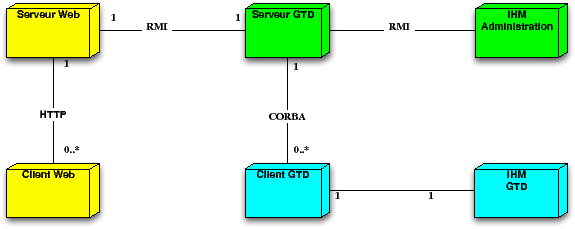
\includegraphics[scale=0.8]{archi.png}
\caption{Architecture Générale}
\end{center}
\end{figure}


Il faut savoir que l'idée intiale de notre projet consistait à simplement implémenter une interface Web, aucune persistance et donc base de données était nécessaire. La seule raison d'être de notre serveur était d'éventuellement allèger la charge du serveur. Nous avons donc rajouter un deuxième serveur en parallèle : ToodleDo qui est disponible gratuitement sur internet.
Ce service comporte évidemment beaucoup de similitude avec le serveur principal (Serveur GTD du schéma ci-dessus).
\\
Afin de gérer de manière uniforme les différents appels vers ces deux serveurs, nous avons défini une interface IServeur qui comporte l'ensemble de ces comportements communs. Toute la partie technique est différenciée lors de l'implémentation de l'interface. Chaque serveur redéfini l'ensemble de ces méthodes avec la partie technique de l'appel. On a à faire à un design pattern Stratégie qui standardise les 2 serveurs.
\\

Le schéma suivant illustre tous les types de communications, tous les protocoles utilisés dans notre architecture.

\begin{figure}[H]
\begin{center}
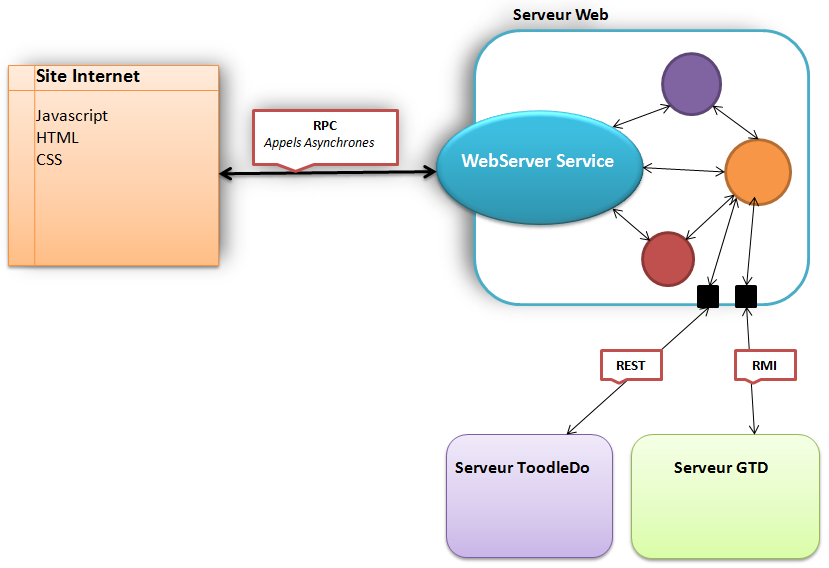
\includegraphics[scale=0.7]{commDansArchi.png}
\caption{Les communications dans l'Architecture Générale}
\end{center}
\end{figure}

\chapter{IHM vers serveur Web}

Notre client léger est developpé à l'aide de la technologie Google Web Toolkit. GWT est un ensemble d'outils logiciels développé par Google, permettant de créer et maintenir des applications web dynamiques dont le client est compilé finalement en Javascript,HTML et css, et dont le serveur est un servlet en code java standard. La particularité de GWT est de fournir sdk de développement  entièrement en java, qui émule les fonctions javascript qui seront utilisées une fois l'application compilée pour être mise en production.Ainsi on developpe en java, on test en java, mais seul le code serveur (tout ce qui se situe dans le package com.alma.serveur) reste en java. Tout ce qui se situe dans le package com.alma.client sera transformé en javascript. Ainsi, on utilise RPC pour communiquer entre le client javascript executé dans le navigateur et le service java executé sur le serveur.\\
Il faut savoir que lors de la création d'un projet avec GWT, la création d'un client et d'un serveur est obligatoire. Dans notre cas cela nous convient parfaitement et permet de rentrer dans les spécifications du projet.
\\ \indent
Une interface distante asynchrone est définie pour permettre au client d'intéragir avec le serveur. En effet, il n'est pas encore possible pour le moment d'utiliser d'interfaces synchrones, non pas parce que Google ne l'a pas prévu, mais tout simplement par choix de conception. Il s'avère que les navigateurs actuels fonctionnent en mono-coeur (pour chaque onglet) et la gestion de requêtes synchrones ne serait pas optimale ce qui provoquerait ralentissement de la machine et du chargement de la page.
\\ \indent
Il faut donc deux flux de communication, le premier direct vers le serveur pour émettre les requêtes, le second asynchrone pour recevoir les réponses du serveur. Pour l'appel d'une méthode, le mécanisme repose sur la définition d'un stub qui permettra l'appel distant. Pour la réponse le design pattern Callback est utilisé. Son utilisation est simple, il suffit de définir une classe dans laquelle deux méthodes sans retour nommées onSuccess et onFailure y sont présentes. Chacune permettant un traitement suivant la réussite ou l'échec de l'appel.
\\ \indent

Pour illustrer ceci, voici un schéma succint présentant l'architecture d'une application écrite en GWT :
\begin{figure}[H]
\begin{center}
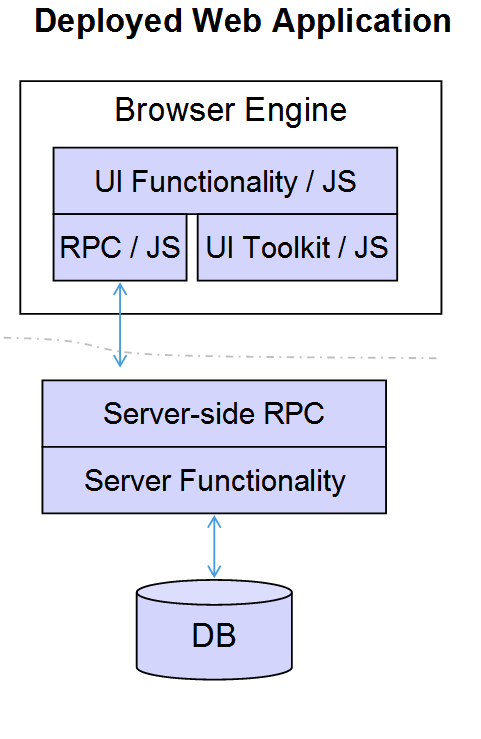
\includegraphics[scale=0.5]{gwt.png}
\caption{Architecture Générale d'une application GWT}
\end{center}
\end{figure}

Les différents appels s'effectuent à l'aide du Javascript qui transmet les appels à l'aide du protocole SOAP. Cette étape est automatiquement géré par l'outil GWT, en effet lors de la compilation du projet, des classes souches (stub) permettent de faire la liaison entre la classe cliente et l'interface asynchrone du serveur.

\chapter{Serveur Web vers ToodleDo}

La documentation fournie par ToodleDo nous informe que la seule façon de communiquer avec leur service se fait à l'aide d'appel de méthodes en REST. \\
REST est un style d'architecture, pas un standard. Il n'existe donc pas de spécifications de REST. Il faut comprendre le style REST et ensuite concevoir des applications ou des services Web selon ce style.
\bigskip
Chaque méthode est appelée à l'aide d'une URL bien spécifique :

\begin{verbatim}
http://exemple.org/maMethode?p1=v1&p2=v2
\end{verbatim}

Si l'on souhaite prendre un exemple concret sur ToodleDo, pour pouvoir ajouter un contexte il faut envoyer une requête à l'adresse suivante :
\begin{verbatim}
http://api.toodledo.com/api.php?method=addContext;key=YourKey;title=MyContext
\end{verbatim}

La clé permet de savoir à quel client la requête est adressée. On peut observer que la méthode est donnée à l'aide du paramètre "method" et son nom grâce au paramètre "title".
\bigskip
Le serveur ToodleDo lance alors la méthode addContext() correspondante et renvoie un flux XML en sortie. Si tout se passe bien il renvoit le noeud suivant :
\begin{verbatim}
<added>12345</added>
\end{verbatim}

Toutes les méthodes fonctionnent sur ce principe d'appel : requête http et réponse avec un flux XML.

\chapter{Serveur Web vers Serveur GTD}

Le type de communication entre notre serveur Web et le serveur GTD est imposé par le sujet. Nous devons obligatoirement communiquer avec les objets distants à l'aide de l'API RMI.
\\
Pour illustrer cela, voici un diagramme montrant l'interaction entre deux applications de types client/serveur :\\

\begin{figure}[H]
\begin{center}
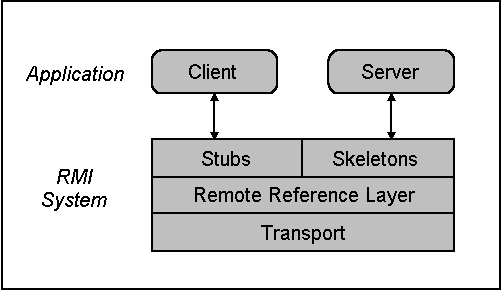
\includegraphics[scale=0.5]{rmi.png}
\caption{Remote Method Invocation}
\end{center}
\end{figure}

Lorsque notre serveur Web souhaitera interroger des méthodes du serveur GTD, il utilisera un objet souche nommé stub sur lequel tous les appels seront effectués. Ce dernier se chargera donc de router les appels sur l'objet squelette (côté serveur GTD) qui interrogera le bon objet distant.
\bigskip
Le groupe chargé de développer le serveur GTD principal a fait le choix d'effectuer des requêtes asynchrones. Leur mise en oeuvre est identique à celle de Google puisqu'il se base sur le même design pattern. Tous nos traitements en retour sont donc effectués à l'aide de l'objet Callback. Cependant une différence subsiste puisque notre objet callback n'est pas sérialisé. Il est considéré comme un objet distant pour le serveur GTD. De ce fait il doit implémenter l'interface Remote (mécanisme RMI) et se disponible sur le réseau. Pour que le serveur GTD puisse faire appel à nos méthodes, on passe dans chaque méthode un objet CallBack qui correspond à un stub. De cette manière ils ont juste à appeler la bonne méthode sur l'objet (onSuccess() ou onFailure()).


\chapter{Sécurité}

Ce chapitre traite de la sécurisation de l'application. 

\section{Demande de connexion au serveur Web}

Lorsqu'un client souhaite utiliser l'application, il doit préalablement s'identifier auprès du système. Elle s'effectue grâce au protocole HTTPS qui permet de crypter les données échangés entre le client et le serveur Web. 
\bigskip
Lorsqu'une connexion est demandée, un objet Session est créé. Celui-ci stocke l'ensemble des informations de connexion aux deux serveurs. En retour, l'identification de cette session est renvoyée au client et c'est avec cet identifiant qu'il pourra exécuter des actions sur le serveur web. Il sera transmis lors de l'appel d'une méthode. Une vérification de la validité de la session est effectuée avant chaque action autre que connection().

\section{Demande de connexion au serveur ToodleDo et GTD}

Le fonctionnement est similaire à notre serveur Web, un jeton pour le serveur ToodleDo et un autre pour le serveur principal GTD est créé lors d'une connexion. Ils permettent d'identifier chaque client/connexion. 
Toute la sécurité repose sur ce principe dans la communication des informations. En effet l'architecture REST de ToodleDo ne permet pas de crypter les paramètres transmis.

\chapter{Conclusion}

L'utilisation d'appel distants au sein du projet nous a permis de mieux comprendre les concepts et mécanismes mis en oeuvre par ces technologies. Nous avons pu constater que leurs utilités étaient réelles dans le développement d'une application client/serveur. Malheureusement, nous n'avons pas pu tester les appels à l'aide de CORBA.\\ Ce projet a donc été l'occasion de développer de nouvelles compétences.
